\documentclass[12pt,letterpaper]{report} % 'letterpaper' es el estándar en Chile

% --- Paquetes de Idioma y Fuentes ---
\usepackage[utf8]{inputenc}   
\usepackage[T1]{fontenc}      
\usepackage[spanish, es-tabla]{babel} % 'es-tabla' para que diga "Tabla" y no "Cuadro"

% --- Formato de Página (Márgenes sugeridos para tesis) ---
\usepackage[left=3.5cm, right=2.5cm, top=2.5cm, bottom=2.5cm]{geometry}
\usepackage{amsmath}

% --- Gráficos y Multimedia ---
\usepackage{graphicx}
\graphicspath{ {./imagenes/} }
\usepackage{caption} % Para mejores leyendas en fotos y tablas

% --- Enlaces y PDF ---
\usepackage[colorlinks=true, allcolors=black]{hyperref} % Hipervínculos en el índice

\usepackage{float}
\usepackage{tikz}
\usepackage{schemabloc}
\usetikzlibrary{arrows.meta, positioning, calc,babel}

% --------------------------------------------------------------------------
% INICIO DEL DOCUMENTO
% --------------------------------------------------------------------------
\begin{document}

% 1. Portada (Se recomienda \input para evitar saltos de página extraños)
\begin{titlepage}
    \begin{center}
        % Logo de la Universidad (asegúrate de tener el archivo del logo en tu carpeta)
        
\includegraphics[width=0.3\textwidth]{imagenes/logo_utal.png} 
        
        \vspace{1cm}
        {\bfseries\Large UNIVERSIDAD DE TALCA \par}
        {\large FACULTAD DE INGENIERÍA \par}
        {\large ESCUELA DE INGENIERÍA CIVIL MECATRÓNICA \par}
        
        \vspace{2.5cm}
        
        % Título de la Tesis
        {\huge\bfseries Aplicación de un control sin sensores para motores stepper aplicado a un Clinostato de 2 dimensiones \par}
        
        \vspace{2cm}
        
        {\large Memoria para optar al Título de \par}
        {\large\bfseries Ingeniero Civil Mecatrónico \par}
        
        \vfill
        
        % Información de los profesores y autor
        \begin{flushright}
            {\large \textbf{Profesor guía:} Dr. Fernando Fuentes \par}
            {\large \textbf{Profesor co-guía:} Dr. Ignacio Torres \par}
            \vspace{0.5cm}
            {\large \textbf{Alumno:} Damián Andrés Bravo Campusano \par}
        \end{flushright}
        
        \vfill
        
        {\large CURICÓ - CHILE \par}
        {\large Primer Semestre 2026 \par}
    \end{center}
\end{titlepage}

% 2. Numeración romana para preliminares (índices, agradecimientos, resumen)
\pagenumbering{roman}

\tableofcontents 
\newpage
\listoffigures 
\newpage
\listoftables
\newpage

% 3. Numeración arábiga para el cuerpo de la tesis
\pagenumbering{arabic}

% Capítulos (usa \include para que cada capítulo empiece en página nueva)
% ============================================================
% CAPÍTULO 1: INTRODUCCIÓN
% ============================================================

\chapter{Introducción}


% ------------------------------------------------------------
\section{Descripción del problema}
% ------------------------------------------------------------

% PÁRRAFO 1: CONTEXTO GENERAL
% Introducir los accionamientos eléctricos y su importancia.
% Hablar brevemente de la evolución desde máquinas de CC hacia
% máquinas de CA gracias al desarrollo de electrónica de potencia
% y procesadores digitales.
% Explicar que muchas aplicaciones requieren control preciso de
% velocidad y/o posición.
%
% NO entrar todavía en clasificación detallada de motores.
% NO incluir ecuaciones.


Los motores eléctricos son máquinas que transforman energia electrica en movimiento mecánico, por lo que son usadas en un sinfin de aplicaciones. Inicialmente, se utilizaban motores de corriente continua, sin embargo, con el avance de dispositivos electrónicos, controladores y procesadores digitales, se ha optado por utilizar máquinas de corriente alterna. Si bien su control es más complejo, pueden llegar a ser menos costosos, con mayor potencia, mejor respuesta dinámica,velocidad máxima, mantenimiento,entre otros factores. \cite{vierbergenPredictingImprovingBehaviour} \cite{deangeloControlParaMaquinas2004}.

A medida que ha avanzado la tecnología,la necesidad de precisión ha crecido también.
Para esto  se suele usar un sensor de posición ó velocidad para cerrar el lazo de control y maximizar la precisión de velocidad ó posición. Sin embargo, hay aplicaciones dónde por la naturaleza del sistema, se necesita un control preciso y constante sin estos sensores. 



% PÁRRAFO 2: INTRODUCCIÓN AL MOTOR PASO A PASO
% Reducir el problema general hacia los motores paso a paso.
% Explicar por qué son atractivos:
%   - Movimiento incremental.
%   - Posibilidad de controlar posición mediante excitación eléctrica.
%   - Operación tradicional a lazo abierto.
%   - Simplicidad y costo.
%   - Uso en aplicaciones de posicionamiento y baja velocidad.
%
% Solo introducir el stepper.
% La clasificación VR / PM / híbrido va en el Marco Teórico.

Para ello, salen alternativas cómo los motores paso a paso(de ahora en adelante, steppers), que pueden mejorar esta precisión a lazo abierto mediante la aplicación de pasos eléctricos.Estos motores, son motores que tienen un movimiento incremental,es decir, que tiene pequeños incrementos angulares discretos, ó pasos. Esto se realiza mediante un cambio ó excitación de las fases de este tipo de motor.
Por esto mismo, este tipo de motor se utiliza bastante, puesto que, puede comandarse en lazo abierto .Adicionalmente, la facilidad de su uso mediante drivers, librerías, y su fácil mantenimiento y costo lo hacen bastante atractivo para la industria ó proyectos de por si.



% PÁRRAFO 3: LIMITACIONES DEL CONTROL A LAZO ABIERTO
% Explicar que la posición eléctrica impuesta no garantiza que
% el rotor siga perfectamente la referencia.
%
% Introducir problemas como:
%   - Perturbaciones de carga.
%   - Variaciones paramétricas.
%   - Pérdida de pasos.
%   - Oscilaciones.
%   - Resonancias.
%   - Ripple de velocidad y/o par.
%
% Destacar que estos efectos son relevantes cuando se requiere
% movimiento suave y preciso, especialmente a baja velocidad.

Aunque estos motores tienden a presentar una alta capacidad de torque, su precisión tanto en velocidad como en posición puede variar dependiendo de las perturbaciones. Al aplicar una velocidad de pasos para un motor sin carga no es lo mismo que aplicar la misma velocidad pero con carga del 50,70 ó 100 \%.
Esto se puede traducir en una pérdida de pasos, oscilaciones, ripple en la velocidad,etc.
Una forma que se realiza para reducir este tipo de desconocimiento de parámetros ó perturbaciones, es aplicar la mayor capacidad de corriente independiente de la carga, intentando realizar un control con todo el potencial eléctrico. Esto no asegura necesariamente que no haya perdida de pasos, además de aumentar el consumo de corriente, aumentar temperatura y disminuir el tiempo de vida del motor.
Estos efectos son tema de estudio para contrarrestarse y lograr un movimiento suave y preciso, especialmente a baja velocidad, dónde las perturbaciones afectan la velocidad comaprado a alta velocidad,situación dónde se podrían hasta despreciar.


% PÁRRAFO 4: CONTROL EN LAZO CERRADO
% Introducir el control realimentado como solución a las
% limitaciones anteriores.
%
% Explicar que conocer la posición y/o velocidad real del rotor
% permite:
%   - Mejorar precisión.
%   - Rechazar perturbaciones.
%   - Evitar pérdida de sincronismo.
%   - Mejorar desempeño dinámico.
%
% Mencionar encoder/resolver únicamente como ejemplos.

Para contrarrestar esto,se suelen colocar encoders ó sensores de posición, los cuales pueden aumentar esta necesitada precisión, rechazar perturbaciones, mejorar el desempeño,etc. Pero estos sensores se traducen en mayor costo, cableado, mantenimiento, y pierde una de las ventajas de los motores paso a paso comparado a otro motor de CA, que es el poder óperar a lazo abierto.

% PÁRRAFO 5: PROBLEMA DE LOS SENSORES MECÁNICOS
% Explicar las desventajas de utilizar sensores:
%   - Mayor costo.
%   - Cableado adicional.
%   - Mayor volumen.
%   - Complejidad de integración.
%   - Mantenimiento.
%   - Confiabilidad en ciertos ambientes.
%
% Este párrafo debe conducir naturalmente hacia el concepto
% de control sensorless.


% PÁRRAFO 6: CONTROL SENSORLESS
% Introducir el control sin sensores mecánicos.
%
% Explicar conceptualmente que posición y velocidad pueden
% estimarse utilizando:
%   - Tensiones.
%   - Corrientes.
%   - Modelo matemático de la máquina.
%   - Observadores/estimadores.
%
% Se puede mencionar el EKF como una alternativa existente,
% pero SIN desarrollar todavía sus ecuaciones.

Sin embargo, hay técnicas que permiten observar y/ó estimar la velocidad de un motor de CA. Para esto, es necesario realizar una medición de algunas variables del motor, tales cómo el voltaje, corriente, algunos parámetros de la máquina y desarrollar un observador ó estimador apropiado.

% PÁRRAFO 7: PROBLEMA SENSORLESS A BAJA VELOCIDAD
% Este es uno de los puntos centrales de la problemática.
%
% Explicar:
%   - Disminución de la FEM a baja velocidad.
%   - Menor información disponible para estimar estados mecánicos.
%   - Problemas de observabilidad.
%   - Mayor sensibilidad frente a errores de modelo.
%   - Mayor efecto relativo del ruido y las perturbaciones.
%
% Respaldar estas afirmaciones con papers.
%
% Conducir hacia la idea de que el control sensorless a baja
% velocidad continúa siendo una condición desafiante.

Una de las problemáticas de observar las variables de un motor se presenta al observar con una baja velocidad mecánica, debido a la disminución de la FEM, puesto que depende de la velocidad del rotor, disminuyendo la información disponible para la estimación de los estados del motor. Por ende, las señales utilizadas presentar una menor relación señal-ruido y es más sensible a perturbaciones, ruido de mediciones y errores de modelo. Esto dificulta distinguir si las variables observadas corresponden al comportamiento real del sistema ó a ótros efectos, deteriorando la estimación de las variables. Sin embargo, hay técnicas de estimación que permiten extender este limite inferior de observabilidad, aumentando las corrientes de flujo  ó campo eléctrico, sin embargo, esto no asegura la observabilidad a velocidad zero. \cite{wangParameterRobustnessImprovement2026}.

% PÁRRAFO 8: PERTURBACIONES PERIÓDICAS Y RIPPLE
%
% IDEA:
% Hasta este punto se estableció que la estimación sensorless se vuelve
% más compleja a baja velocidad. Ahora introducir una segunda problemática:
% las perturbaciones periódicas propias de la máquina.
%
% ORDEN RECOMENDADO:
%
% 1. Explicar que el torque desarrollado por una máquina real no es
%    perfectamente constante, sino que puede contener componentes
%    periódicas.
% 2. Introducir el concepto de torque ripple como las oscilaciones
%    del torque alrededor de su valor medio.
%
% 3. Explicar que estas oscilaciones pueden tener distintos orígenes:
%       - geometría de la máquina;
%       - armónicos electromagnéticos;
%       - conmutación/excitación;
%       - interacción rotor-estator;
%       - detent torque.
%
% 4. Particularizar hacia motores paso a paso.
%    Introducir el detent torque como una perturbación periódica
%    asociada a la posición del rotor que puede existir incluso
%    cuando las fases no están energizadas.
%
% 5. Explicar la consecuencia mecánica:
%
%       perturbación periódica de torque
%                     ↓
%             oscilación de torque
%                     ↓
%             ripple de velocidad
%
% 6. Conectar esto con BAJA VELOCIDAD:
%    a bajas velocidades, estas perturbaciones pueden adquirir
%    mayor importancia relativa respecto del torque requerido
%    para mantener el movimiento.
%
% 7. Finalmente conectar con SENSORLESS:
%    si la velocidad utilizada por el controlador proviene de un
%    observador, la perturbación afecta a la planta mientras que
%    la compensación depende de variables mecánicas estimadas.
%
% IMPORTANTE:
% No desarrollar todavía la ecuación sinusoidal del detent torque.
% Eso corresponde al marco teórico/modelado.
%
% Tampoco afirmar todavía que el detent torque es "la principal"
% causa del ripple. Eso deberá justificarse bibliográficamente.
La capacidad de un motor para generar torque sin variaciones de carga es idealmente constante, pero la realidad es algo diferente. Dentro de las propiedades internas existen ciertas configuraciones propias del motor que pueden generar componentes periódicos en el torque generado por el motor. A estas oscilaciones se les llama como torque ripple, las cuales pueden ser generadas por distintas variables, cómo la geometría del motor, armónicos electromagnéticos, el tipo de conmutación, interacción rotor-stator o torque de detención. Muchas de estas perturbaciones son en función de la posición, por lo tanto,están presente independiente de si el motor está energizado ó no. Los motores stepper son capaces de generar pasos con precisión, en gran medida gracias a estas características,puesto que son construidos pensados aprovechando este tipo de diseño. 

Durante el movimiento del rotor, estas componentes periódicas de torque pueden producir oscilaciones en la velocidad del motor.Estos efectos pueden aumentar a baja velocidad, dónde las variaciones pueden ser mucho más significativas, deteriorando el comportamiendo de velocidad.Debido a la diversidad de fenómenos que pueden contribuir a estas oscilaciones,el presente trabajo se centrará específicamente en la componente
periódica asociada al \textit{cogging torque}, estudiando su efecto
sobre la velocidad del motor y su posterior compensación.

En cuestión del cogging, este se suele compensar para disminuir ó eliminar sus efectos. En la literatura, las principales formas de compensación son:


\begin{enumerate}
    \item \textbf{Métodos pasivos:} corresponden a modificaciones
    constructivas de la máquina destinadas a reducir la perturbación
    desde su origen, tales como modificaciones en la geometría del
    rotor o estator.

    \item \textbf{Métodos activos:} utilizan estrategias de control
    para reducir o compensar el efecto de la perturbación durante
    el funcionamiento del motor. Estos métodos pueden clasificarse
    a su vez en:

    \begin{enumerate}
        \item \textbf{Métodos offline:} la perturbación es caracterizada
        o identificada previamente, utilizando posteriormente esta
        información durante la operación del motor.

        \item \textbf{Métodos online:} la perturbación es estimada o
        identificada durante el funcionamiento del motor, permitiendo
        adaptar la acción de compensación a las condiciones de operación.
    \end{enumerate}
\end{enumerate}


% PÁRRAFO 9:
% Introducir de manera GENERAL las alternativas de compensación.
%
% Puedes separar conceptualmente:
%
% 1. MÉTODOS PASIVOS / CONSTRUCTIVOS
%    Modifican el diseño de la máquina para reducir la generación
%    de la perturbación.
%
%    Ejemplos:
%       - geometría del rotor/estator;
%       - modificación de dientes;
%       - skewing;
%       - optimización electromagnética.
%
% 2. MÉTODOS ACTIVOS / DE CONTROL
%    No modifican físicamente la máquina, sino que intentan
%    contrarrestar la perturbación mediante el accionamiento.
%
%    Ejemplos generales:
%       - modificación de las referencias de corriente;
%       - compensación feedforward;
%       - control resonante;
%       - observadores de perturbación.
%
% Dentro de las estrategias activas puedes introducir otra
% clasificación importante para TU tesis:
%
%       OFFLINE                     ONLINE
%          |                           |
% identificación previa       estimación/adaptación
% de la perturbación          durante el funcionamiento
%          |                           |
% LUT / mapa / perfil         observador / estimador /
% predefinido                 compensación adaptativa
%
%
% IMPORTANTE:
% En esta sección NO hacer todavía una revisión paper por paper.
%
% Solo quieres demostrar:
%
% "El problema existe y hay distintas formas de abordarlo,
% pero algunas requieren conocimiento previo de la perturbación
% o información mecánica del rotor."
%
% Esto prepara directamente el problema específico de tu tesis.

% ============================================================
\section{Antecedentes del tema}
% ============================================================

% Esta sección corresponde principalmente al ESTADO DEL ARTE.
% Aquí se utilizan los papers seleccionados para mostrar:
%
%   1. Qué se ha hecho.
%   2. Cómo se ha hecho.
%   3. Qué resultados se han obtenido.
%   4. Qué limitaciones permanecen.
%
% Debe conducir progresivamente hacia el GAP de investigación.


% ------------------------------------------------------------
\subsection{Control de motores paso a paso}
% ------------------------------------------------------------

% Revisar trabajos relacionados con:
%   - Control tradicional de steppers.
%   - Microstepping.
%   - Control de corriente.
%   - Control de velocidad.
%   - Control de posición.
%   - Control vectorial / FOC aplicado a steppers.
%   - Lazo abierto versus lazo cerrado.
%
% El objetivo NO es explicar matemáticamente cada estrategia.
% El objetivo es mostrar la evolución de las técnicas de control.


% ------------------------------------------------------------
\subsection{Control sensorless de motores paso a paso}
% ------------------------------------------------------------

% Revisar específicamente los métodos sensorless encontrados
% en la literatura.
%
% Por ejemplo:
%   - Métodos basados en FEM.
%   - Observadores de estado.
%   - EKF.
%   - Sliding Mode Observer.
%   - MRAS, si aparece en tus papers.
%   - HFI/LFI.
%   - Métodos basados en saliencia.
%
% Comparar:
%   - Qué estiman.
%   - Qué variables utilizan.
%   - Rango de velocidad.
%   - Requerimientos.
%   - Limitaciones.
%
% Esta subsección debería conducir hacia:
%
%       SENSORLESS
%           ↓
%   PROBLEMAS A BAJA VELOCIDAD


% ------------------------------------------------------------
\subsection{Control sensorless a baja velocidad}
% ------------------------------------------------------------

% Hacer zoom específicamente en la región de baja velocidad.
%
% Revisar:
%   - Problemas de observabilidad.
%   - Disminución de FEM.
%   - Saliencia.
%   - HFI.
%   - LFI.
%   - Observadores no lineales.
%   - EKF a baja velocidad.
%
% Analizar hasta qué velocidad trabajan los papers.
%
% Esto es especialmente importante para justificar por qué
% estudiar aproximadamente 1--10 rad/s (o el rango definitivo
% de la tesis) constituye un problema relevante.


% ------------------------------------------------------------
\subsection{Perturbaciones periódicas y ripple}
% ------------------------------------------------------------

% Revisar literatura relacionada con:
%   - Detent torque.
%   - Cogging torque.
%   - Torque ripple.
%   - Armónicos espaciales.
%   - Ripple de velocidad.
%
% Analizar:
%   - Origen físico.
%   - Dependencia con posición.
%   - Dependencia con velocidad.
%   - Frecuencias características.
%   - Modelos utilizados en los papers.
%
% Se pueden mencionar representaciones sinusoidales/Fourier,
% pero el desarrollo matemático detallado debe quedar para
% el Marco Teórico.


% ------------------------------------------------------------
\subsection{Métodos de reducción y compensación del ripple}
% ------------------------------------------------------------

% Revisar las estrategias encontradas para reducir ripple.
%
% Una forma útil de organizar esta sección sería:
%
% A) MÉTODOS OFFLINE
%   - Look-up tables.
%   - Mapas de compensación.
%   - Perfiles de corriente preidentificados.
%   - Identificación previa de armónicos.
%
% B) MÉTODOS ONLINE
%   - Observadores de perturbación.
%   - Estimadores de torque.
%   - Métodos adaptativos.
%   - Control resonante.
%   - Estimación armónica online.
%
% Para cada paper interesa identificar:
%   - ¿Usa sensor mecánico?
%   - ¿Es sensorless?
%   - ¿Trabaja a baja velocidad?
%   - ¿Estima la perturbación?
%   - ¿La compensación es online?
%   - ¿Reduce ripple de velocidad o de torque?
%   - ¿Requiere conocer previamente la perturbación?


% ------------------------------------------------------------
\subsection{Brecha de investigación}
% ------------------------------------------------------------

% Esta subsección debe ser el resultado de TODA la revisión anterior.
%
% La lógica esperada sería:
%
%   CONTROL DE STEPPERS
%          ↓
%   CONTROL SENSORLESS
%          ↓
%   BAJA VELOCIDAD
%          ↓
%   PERTURBACIONES PERIÓDICAS
%          ↓
%   COMPENSACIÓN DEL RIPPLE
%          ↓
%   ESTIMACIÓN/COMPENSACIÓN ONLINE
%          ↓
%        GAP
%
% El GAP debe construirse exclusivamente a partir de lo que
% realmente indiquen los papers revisados.
%
% Hipótesis preliminar del GAP:
%
% "Existe una oportunidad de desarrollar estrategias capaces
% de estimar y compensar en línea perturbaciones periódicas en
% accionamientos stepper sensorless operando a baja velocidad,
% utilizando las variables estimadas por el propio sistema de
% observación para reducir el ripple de velocidad."
%
% NO dejar esta frase definitiva hasta terminar la comparación
% de los papers seleccionados.



% ============================================================
\section{Objetivos}
% ============================================================


% ------------------------------------------------------------
\subsection{Objetivo general}
% ------------------------------------------------------------

% Debe responder directamente al GAP identificado.
%
% Versión preliminar:
%
% "Desarrollar una estrategia de control sensorless para un motor
% paso a paso que permita estimar y compensar en línea perturbaciones
% periódicas, con el propósito de reducir el ripple de velocidad
% durante la operación a baja velocidad."


% ------------------------------------------------------------
\subsection{Objetivos específicos}
% ------------------------------------------------------------

% Los objetivos específicos deberían seguir la metodología real
% de la tesis.
%
% Posible secuencia:
%
% 1. Modelar matemáticamente el motor paso a paso considerando
%    las perturbaciones periódicas relevantes.
%
% 2. Implementar una estrategia de estimación sensorless de
%    las variables mecánicas del motor.
%
% 3. Caracterizar el efecto de las perturbaciones periódicas
%    sobre la velocidad y sobre el estimador.
%
% 4. Desarrollar un método para estimar en línea la perturbación.
%
% 5. Diseñar una estrategia para compensar la perturbación estimada.
%
% 6. Integrar el estimador y el compensador dentro del sistema
%    de control sensorless.
%
% 7. Evaluar la reducción del ripple y el desempeño del sistema
%    mediante simulaciones y/o validación experimental.



% ============================================================
\section{Contribuciones de esta memoria}
% ============================================================

% Aquí NO repetir simplemente los objetivos.
%
% Los objetivos dicen:
%       "qué se pretende hacer".
%
% Las contribuciones dicen:
%       "qué aporta este trabajo respecto al estado del arte".
%
% Posibles contribuciones, sujetas a los resultados finales:
%
%   - Estrategia de estimación online de perturbaciones periódicas.
%
%   - Integración de dicha estimación con un esquema sensorless
%     basado en EKF.
%
%   - Compensación de perturbaciones sin utilizar medición mecánica
%     directa de posición o velocidad.
%
%   - Reducción del ripple de velocidad durante operación
%     a baja velocidad.
%
%   - Análisis del efecto del desfase/error del observador sobre
%     la compensación.
%
%   - Comparación cuantitativa entre operación con y sin
%     compensación.
%
% IMPORTANTE:
% Dejar únicamente las contribuciones que finalmente puedan
% demostrarse mediante resultados.



% ============================================================
\section{Organización de la memoria}
% ============================================================

% Describir brevemente qué contiene cada capítulo.
%
% Ejemplo:
%
% Capítulo 1:
% Introducción, problemática, antecedentes, brecha de investigación,
% objetivos y contribuciones.
%
% Capítulo 2:
% Fundamentos teóricos y modelo matemático del motor paso a paso.
%
% Capítulo 3:
% Desarrollo de la estrategia de control y estimación sensorless.
%
% Capítulo 4:
% Desarrollo de la estrategia de estimación y compensación
% de perturbaciones periódicas.
%
% Capítulo 5:
% Resultados, comparación de estrategias y discusión.
%
% Capítulo 6:
% Conclusiones y líneas de trabajo futuro.



% ============================================================
% CAPÍTULO 2: MARCO TEÓRICO
% ============================================================

\chapter{Marco teórico}


% ------------------------------------------------------------
\section{Motores eléctricos}
% ------------------------------------------------------------

% AQUÍ sí introducir formalmente los tipos de motores.
%
% Hacer una clasificación breve para llegar rápidamente al stepper.
% No transformar esta sección en una revisión general de todas
% las máquinas eléctricas.


% ------------------------------------------------------------
\section{Motores paso a paso}
% ------------------------------------------------------------

% Explicar:
%   - Principio de funcionamiento.
%   - Construcción.
%   - Rotor y estator.
%   - Número de polos/dientes.
%   - Paso mecánico.
%   - Excitación de fases.


% ------------------------------------------------------------
\subsection{Tipos de motores paso a paso}
% ------------------------------------------------------------

% Aquí colocar:
%   - Reluctancia variable (VR).
%   - Imán permanente (PM).
%   - Híbrido (HB).
%
% Explicar diferencias constructivas y justificar cuál se utiliza
% en esta memoria.


% ------------------------------------------------------------
\section{Modelo matemático del motor paso a paso}
% ------------------------------------------------------------

% Aquí comienza el desarrollo matemático formal.
%
% Incluir según corresponda:
%   - Modelo eléctrico.
%   - Modelo mecánico.
%   - FEM.
%   - Torque electromagnético.
%   - Inductancias.
%   - Saliencia.


% ------------------------------------------------------------
\section{Transformaciones de coordenadas}
% ------------------------------------------------------------

% Explicar:
%   - alpha-beta.
%   - d-q.
%   - Transformaciones utilizadas.
%   - Significado físico.
%   - Relación entre ángulo eléctrico y mecánico.


% ------------------------------------------------------------
\section{Control vectorial del motor paso a paso}
% ------------------------------------------------------------

% Explicar formalmente:
%   - Control de Id.
%   - Control de Iq.
%   - PI de corriente.
%   - Control de velocidad.
%   - Generación de referencias.
%   - Saturaciones.
%   - MTPA si finalmente forma parte de la estrategia.


% ------------------------------------------------------------
\section{Control sensorless}
% ------------------------------------------------------------

% Fundamentos matemáticos necesarios para comprender el estimador.
%
% Evitar repetir el estado del arte del Capítulo 1.
%
% Capítulo 1:
%   "qué métodos existen y qué hicieron otros autores".
%
% Capítulo 2:
%   "cómo funcionan matemáticamente los métodos que YO necesito".


% ------------------------------------------------------------
\subsection{Filtro de Kalman extendido}
% ------------------------------------------------------------

% Desarrollar:
%   - Modelo de estados.
%   - Predicción.
%   - Corrección.
%   - Matrices Q y R.
%   - Jacobianos.
%   - Estados estimados.
%
% Luego particularizarlo al modelo del stepper.


% ------------------------------------------------------------
\section{Perturbaciones periódicas}
% ------------------------------------------------------------

% Fundamentos físicos y matemáticos.
%
% Incluir:
%   - Cogging/detent torque.
%   - Torque ripple.
%   - Periodicidad respecto a theta_m.
%   - Frecuencia de perturbación respecto a Wm.
%   - Representación mediante series de Fourier.
%
% Aquí sí corresponde desarrollar expresiones como:
%
%       T_d = T_{dm}\sin(N_r\theta_m + \phi)
%
% y posteriormente sus armónicos si son utilizados.


% ------------------------------------------------------------
\section{Compensación de perturbaciones periódicas}
% ------------------------------------------------------------

% Fundamentos matemáticos necesarios para tu propuesta.
%
% Según la versión final:
%   - Control resonante.
%   - PR.
%   - Estimación armónica.
%   - Compensación feedforward.
%   - Compensación adaptativa.
%   - Desfase del sistema.
%
% Esta sección debería entregar las herramientas necesarias para
% entender posteriormente tu metodología propuesta.
 \chapter{Marco teórico}
En esta sección se presenta una revisión de los conceptos fundamentales relacionados con el control de motores paso a paso, así como una descripción de las principales técnicas de control robusto que se han desarrollado para sistemas con perturbaciones no medibles. Se abordarán también los desafíos específicos que plantea el control de un clinostato accionado por motores paso a paso, y se discutirán las estrategias más adecuadas para mitigar los efectos de las perturbaciones mecánicas variables.

\section{Motor Stepper}
Los motores paso a paso son un tipo de motor eléctrico que se caracteriza por su capacidad para dividir una rotación completa en un número finito de pasos, lo que permite un control preciso de la posición y la velocidad a lazo abierto. Estos motores funcionan mediante la excitación secuencial de las bobinas, lo que genera un campo magnético que interactúa con el rotor para producir movimiento. La principal ventaja de los motores paso a paso es su simplicidad y bajo costo, ya que no requieren sensores de posición ni sistemas de retroalimentación para su operación. Sin embargo, esta característica también los hace susceptibles a errores de posición y velocidad cuando se enfrentan a perturbaciones mecánicas o variaciones de carga, lo que puede afectar significativamente su desempeño en aplicaciones críticas como los clinostatos.





\section{Modelado electromecánico del motor}
Un motor paso a paso, puede modelarse como un motor de imanes permanentes.
El modelo electromecánico de un motor paso a paso puede describirse mediante un conjunto de ecuaciones diferenciales que relacionan las variables eléctricas (corrientes y voltajes) con las variables mecánicas (posición, velocidad y torque). En particular, el torque generado por el motor depende de la corriente en las bobinas y de la posición angular del rotor, lo que introduce una no linealidad en el sistema. Además, la presencia de perturbaciones mecánicas variables, como las que se presentan en el clinostato debido a la geometría del sistema de poleas, añade complejidad al modelado y al diseño de controladores robustos.

Una aproximación común para el modelado de motores paso a paso es utilizar un modelo de segundo orden que capture la dinámica del sistema, incluyendo la inercia del rotor, la fricción y las perturbaciones externas. Este modelo puede ser utilizado para analizar la estabilidad del sistema y diseñar controladores que sean capaces de mantener un desempeño adecuado incluso en presencia de perturbaciones no medibles.

\begin{equation}
\label{eq:modelo_motor}
\left\{
\begin{aligned}
    L \frac{d i_{a}}{dt} &= V_{a} - R i_{a} - e_{a}(\theta_{e}) \\
    L \frac{d i_{b}}{dt} &= V_{b} - R i_{b} - e_{b}(\theta_{e}) \\
    J \frac{d \omega_{m}}{dt} &= \tau_{em} - B \omega_{m} - \tau_{dm} - \tau_{load} \\
    \frac{d \theta_{m}}{dt} &= \omega_{m} \\
    \theta_{e} &= \theta_{m} \cdot N_{r}
\end{aligned}
\right.
\end{equation}

\section{Transformada de Park y Clarke}
La transformada de Clarke es una transformada que permite, mediante una multiplicación de matrices, transformar toda la información que hay en un sistema trifásico en un sistema bifásico. Esta transformada es bastante útil, puesto que reduce la cantidad de información redundante, y adicionalmente, la salida de esta transformada es una salida ortogonal ( es decir, son dos señales separadas en 90 grados). Debido a que nuestro motor stepper es bifásico, ya desfasado 90 grados, esta transformada se descarta como una opción para el control, pero es importante conocerla, puesto que es la base de la transformada de Park, que sí se utiliza en el control de motores paso a paso.

La transformada de park tiene como objetivo transformar un sistema de referencia estacionario, a un sistema de referencia rotatorio.Esto es útil, puesto que en un sistema electrico alterno, existe información redundante en una gráfica sinoidal, dónde los valores más importantes serían la frecuencia y la amplitud, pero no el valor instantáneo. Al transformar a un sistema de referencia rotatorio, se obtiene una recta si la amplitud se mantiene constante, lo que facilita el análisis y el control del sistema. Además, esta transformada permite separar la información de torque y flujo en dos componentes ortogonales, lo que es fundamental para el diseño de controladores basados en la regulación de corrientes.

\begin{equation}
    \begin{bmatrix}
        i_d \\
        i_q
    \end{bmatrix} = 
    \begin{bmatrix}
        \cos(\theta) & \sin(\theta) \\
        -\sin(\theta) & \cos(\theta)
    \end{bmatrix}
    \begin{bmatrix}
        i_{\alpha} \\
        i_{\beta}
    \end{bmatrix}
\end{equation}

Otra de las ventajas que se tiene al utilizar esta transformada, es el ahorro computacional, puesto que se calcula solo una vez las funciones de seno y coseno, y luego se utilizan para calcular las señales de control, lo que es especialmente relevante en sistemas embebidos con recursos limitados.

\section{FOC en motores steppers}
Field orient control (FOC) es una técnica de control vectorial que se utiliza para controlar motores eléctricos, incluyendo motores paso a paso. Esta técnica se basa en la idea de controlar el flujo magnético y el torque del motor de manera independiente, lo que permite obtener un desempeño dinámico superior y una mayor eficiencia energética. En el caso de los motores paso a paso, el FOC se implementa utilizando la transformada de Park para separar las corrientes en componentes de flujo y torque, lo que facilita el diseño de controladores que puedan mantener un desempeño adecuado incluso en presencia de perturbaciones mecánicas variables.

Puesto que nuestro motor tiene solamente 2 fases desfasados en 90 grados,uno puede aplicar de forma inmediata la transformada de Park, y obtener una señal de control para cada fase, lo que simplifica la implementación del FOC. 
Al aplicar la transformada de Park a las ecuaciones (\ref{eq:modelo_motor}), se obtiene un modelo en el dominio de Park que puede ser utilizado para diseñar controladores basados en la regulación de corrientes. 

\begin{equation}
    \begin{bmatrix}
        \dot{I}_d \\
        \dot{I}_q \\
        \dot{\omega_{m}} \\
        \dot{\theta_{m}}
    \end{bmatrix} = 
    \begin{bmatrix}
        (V_{d} - R I_{d})\frac{1}{L} + \omega_{m} L N_{r} I_{q} \\
        (V_{q} - R I_{q} + K_{e}\omega_{m} )\frac{1}{L} - \omega_{m} L N_{r} I_{d} \\
        (K_{e} I_{q} - \tau_{load} - B\omega_{m} - \tau_{dtm} )\frac{1}{J} \\
        \omega_{m}
    \end{bmatrix}
\end{equation}

\section{Observabilidad y controlabilidad}
La observabilidad de un sistema es la propiedad que determina si es posible reconstruir los estados internos de este mismo a partir de un conjunto limitado de mediciones disponibles, tales como la entrada u otras variables propias medibles del mismo sistema. 
La controlabilidad es la propiedad que determina si es posible llevar el sistema a cualquier estado deseado mediante la aplicación de una entrada adecuada. 
Estas propiedades son fundamentales para analizar el comportamiento de un sistema y el diseño de su sistema de control, ya que no todos los sistemas son observables y/o controlables, lo que puede estar limitado según las variables de interés a controlar, las mediciones disponibles y el modelo del sistema. En el caso de un motor paso a paso, la observabilidad y controlabilidad pueden verse comprometidas en ciertas regiones de operación, especialmente a bajas velocidades o en presencia de perturbaciones mecánicas variables, lo que dificulta el diseño de controladores robustos que puedan mantener un desempeño adecuado en estas condiciones.

Dado que, el sistema propuesto es no-lineal, la observabilidad y controlabilidad pueden depender del punto de operación considerado, lo que hace que el análisis de estas propiedades sea más complejo. Para ello, se le llamará observabilidad local a la capacidad de un sistema para ser observable en un punto específico del espacio de estados, lo que puede variar según las condiciones de operación y las perturbaciones presentes. En el caso de un motor paso a paso, la observabilidad local puede verse comprometida en ciertas regiones de operación, especialmente a bajas velocidades o en presencia de perturbaciones mecánicas variables, lo que dificulta el diseño de controladores robustos que puedan mantener un desempeño adecuado en estas condiciones.

La observabilidad local viene dado por la siguiente ecuación:


\begin{equation}
\label{eq: Matriz A y B}
\left\{
\begin{aligned}
 A &= \left. \frac{\partial f}{\partial x} \right|_{x=x_0,u=u_0} \\
 B &= \left. \frac{\partial f}{\partial u} \right|_{x=x_0,u=u_0} \\
\end{aligned}
\right.
\end{equation}

Dónde $f$ representa las ecuaciones del sistema no lineal, $x$ es el vector de estados, $u$ es el vector de entradas, y $x_0$ y $u_0$ son el punto de operación alrededor del cual se realiza la linealización.

La matriz de observabilidad se calcula utilizando la matriz A y la matriz de salida C, mientras que la matriz de controlabilidad se calcula utilizando la matriz A y la matriz B. Para este sistema, se asumió que las salidas disponibles para la medición son la corriente en los ejes d y q, lo que implica que la matriz de salida C es la siguiente:




\begin{equation}
    C = 
    \begin{bmatrix}
        1 & 0 & 0 & 0 \\
        0 & 1 & 0 & 0 \\
    \end{bmatrix}
\end{equation}

 La observabilidad y controlabilidad del sistema se determina evaluando el rango de estas matrices. Si el rango de la matriz de observabilidad es igual al número de estados, entonces el sistema es completamente observable. Si el rango de la matriz de controlabilidad es igual al número de estados, entonces el sistema es completamente controlable.

 Para este caso, la matriz de observabilidad se calcula utilizando la matriz A y la matriz C, y se obtiene la siguiente matriz de observabilidad:

\begin{equation}
    O = 
    \begin{bmatrix}
        C \\
        CA \\
        CA^2 \\
        CA^3 \\
    \end{bmatrix}
\end{equation}

y la de controlabilidad se calcula utilizando la matriz A y la matriz B, y se obtiene la siguiente matriz de controlabilidad:

\begin{equation}
    Q = 
    \begin{bmatrix}
        B & AB & A^2B & A^3B \\
    \end{bmatrix}   
\end{equation}



Utilizando la ecuación \ref{eq: dq}, se utilizaron los siguientes parámetros para linealizar y calcular las matrices de observabilidad y controlabilidad:

\begin{table}[htbp]
    \centering
    \caption{Tabla de parámetros punto de operación}
    \label{tab:punto de operacion}
    \begin{tabular}{|l|c|c|c|c|c|c|c|c|c|c|c|c|c|c|}
        \hline
        \textbf{Parámetro} &  $R $ & Ld  & Lq  & Ke & Kt & J & B & P & $W_{m}$ & $I_{d}$ & $I_{q}$ & $T_{x}$ & $V_{d}$ & $V_{q}$ \\
        \hline
        % Valores de punto de operación (rellenar según corresponda)
        \textbf{Valor} &2.5 & 3.2& 8.1 & 0.045 & 0.045 & 0.01 & 0.11 & 50 & 0.1 & 0 & 1 & 0.2& 0 &10 \\
        \hline
    \end{tabular}
\end{table}

Después de calcular las matrices de observabilidad y controlabilidad, se evaluó su rango para determinar la observabilidad y controlabilidad del sistema.Se utilizó el programa de Matlab como apoyo a esto (\ref{lst:resultados}).  Se encontró que el sistema es parcialmente observable y totalmente controlable, lo que implica que no todos los estados pueden ser estimados,pero si controlados mediante el control de voltaje.

El rango de la matriz de observabilidad se encontró que es igual a 3, lo que indica que el sistema es parcialmente observable, ya que el número de estados es 4. El rango de la matriz de controlabilidad se encontró que es igual a 4, lo que indica que el sistema es totalmente controlable, ya que el número de estados es 4. Esto significa que hay un estado que no puede ser estimado pero si controlado, lo que es consistente con la naturaleza del sistema, puesto que en un motor paso a paso, la posición del rotor no es directamente medible, pero puede ser controlada a través de las corrientes en los ejes d y q. Cabe destacar, que esto es solo para un sistema linealizado alrededor de un punto de operación específico, y la observabilidad y controlabilidad pueden variar dependiendo del punto de operación y de las variables que se estén midiendo y controlando.Por ejemplo, en el punto de operación dado, las derivadas se asumen 0,por lo que no existe información de la posición del rotor, lo que hace que esta no sea observable, pero si se agregaran derivadas no nulas, se podría obtener información de la posición del rotor, lo que haría que esta fuera observable.Adicionalmente, a altas velocidades, la fuerza electro-motriz es más significativa, lo que podría proporcionar información adicional para la estimación de la posición del rotor, lo que también podría mejorar la observabilidad del sistema. Por lo tanto, es importante considerar estos factores al diseñar el EKF y al evaluar la observabilidad y controlabilidad del sistema en diferentes condiciones de operación.

Cómo el objetivo es controlar la velocidad para que sea constante, provocando que las derivadas sean 0 en un punto de operación de baja velocidad,por lo que tampoco existe información del rotor that pueda ser entrega por la fuerza electro-motriz, es necesario aplicar alguna estrategia para mejorar la observabilidad del sistema, como por ejemplo, aplicar una señal de excitación adicional para obtener información de la posición del rotor, lo that permitiría una mejor estimación de los estados y un control más preciso del motor paso a paso.

\section{Filtro de Kalman Extendido}

Dado que una de las principales restricciones del sistema es la imposibilidad de medir directamente la velocidad mecánica, resulta necesario recurrir a técnicas de estimación basadas en observadores de estado. Un observador de estados es una herramienta de control que permite reconstruir variables internas del sistema que no son directamente medibles, a partir de un conjunto limitado de mediciones disponibles y de un modelo matemático que describe la dinámica del sistema.

Dentro de este enfoque, los filtros de Kalman corresponden a una clase de observadores de estado de naturaleza probabilística, los cuales permiten estimar los estados del sistema combinando la información proveniente de las mediciones disponibles, las entradas aplicadas y la predicción del modelo, considerando explícitamente la presencia de ruido y perturbaciones.

Para que un observador de estados sea capaz de reconstruir adecuadamente todas las variables de interés, el sistema debe cumplir ciertas condiciones estructurales, entre ellas la observabilidad. Esta propiedad puede analizarse a través del modelo del sistema y depende del punto de operación considerado, lo que resulta particularmente relevante en sistemas no lineales o con parámetros variables, como los sistemas de accionamiento eléctrico.

Para el caso específico de un motor paso a paso, la observabilidad considerando solo la lectura de variables como las corrientes y el voltaje aplicado, puede verse comprometida en ciertas regiones de operación, especialmente a bajas velocidades o en presencia de perturbaciones mecánicas variables. Esto se debe a que la dinámica del sistema puede volverse menos sensible a las variaciones de los estados internos, lo que dificulta la capacidad del observador para distinguir entre diferentes configuraciones del sistema. En estas condiciones, el diseño de un filtro de Kalman extendido (EKF) puede resultar insuficiente para garantizar una estimación precisa de la velocidad, lo que a su vez afecta el desempeño del controlador basado en esta estimación. Por esta razón, es necesario considerar estrategias adicionales que permitan mejorar la observabilidad del sistema, como la inyección de señales de alta frecuencia.

\section{High Frecuency Injection}
Este método utiliza la inyección de señales de alta frecuencia para mejorar la observabilidad del sistema, especialmente en regiones donde el modelo linealizado no es observable. La idea es introducir una señal de excitación adicional que permita generar una respuesta del sistema que sea sensible a las variaciones de los estados internos, lo que facilita la estimación de variables como la velocidad mecánica.Esta técnica no reconoce especificamente la posición del ángulo eléctrico, si no más bien, identifica el error entre la posición estimada y la posición real, lo que permite corregir la estimación de la velocidad y mejorar el desempeño del controlador. 

Lo que se implementa, es simplementa un voltaje de alta frecuencia en el eje del flujo, lo que genera una corriente de alta frecuencia que puede ser analizada para extraer información sobre la posición del rotor y la velocidad. Si se supone un angulo diferente al real, esto se verá reflejado en la corriente del eje del torque, lo que permite corregir la estimación de la velocidad y mejorar el desempeño del controlador. Esta técnica es especialmente útil en aplicaciones donde se requiere un control preciso a bajas velocidades, como en el caso de los clinostatos, donde las perturbaciones mecánicas variables pueden afectar significativamente el desempeño del sistema.

\begin{equation}
    \begin{bmatrix}
        V_d \\
        V_q
    \end{bmatrix} = 
    \begin{bmatrix}
         V_{dHF} \\
        0
    \end{bmatrix}
\end{equation}

Ya que se implementa una señal de bajo voltaje y de alta frecuencia, la respuesta será  una corriente de alta frecuencia,ya que el sistema mecánico no tendrá el tiempo suficiente para responder a la entrada ,lo que no afecta el desempeño del sistema, pero en caso de que el angulo estimado sea diferente al real, se verá reflejado en la corriente del eje del torque, lo que permite corregir la estimación de la velocidad y mejorar el desempeño del controlador. Pero esta tecnica solo es posible para motores con saliencia, es decir, motores que presentan una diferencia entre la inductancia en el eje del flujo y el eje del torque, lo que permite generar una respuesta de alta frecuencia que sea sensible a las variaciones de la posición del rotor. En el caso de los motores paso a paso, esta condición se cumple debido a su construcción interna, lo que hace que esta técnica sea especialmente adecuada para mejorar la observabilidad y el desempeño del sistema de control en aplicaciones como los clinostatos.

\section{Saliencia}
La saliencia es una propiedad de los motores eléctricos que se refiere a la diferencia entre la inductancia en el eje del flujo y el eje del torque. Esta diferencia permite generar una respuesta de alta frecuencia que sea sensible a las variaciones de la posición del rotor, lo que es fundamental para la implementación de técnicas como la inyección de señales de alta frecuencia para mejorar la observabilidad del sistema. Estos valores de inductancia van cambiando según la posición del rotor, debido a la geometría interna del motor, producto de la diferencia de resistencia que se genera entre el aire y el hierro, lo que hace que la inductancia varíe en función de la posición angular del rotor. 
Los motores paso a paso presentan una saliencia significativamente mayor que los motores PMSM, debido a que presentan una construcción interna de más dientes ó número de polos. Un PMSM típico puede presentar entre 4 a 6 pares de polos, mientras que un motor paso a paso puede presentar entre 50 a 100 pares de polos, lo que genera una diferencia significativa en la inductancia entre el eje del flujo y el eje del torque, lo que hace que esta técnica sea especialmente adecuada para mejorar la observabilidad y el desempeño del sistema de control en aplicaciones como los clinostatos. 

Todos los motores presentan saliencia, pero en algunos casos esta puede ser tan baja que no se puede aprovechar para mejorar la observabilidad del sistema, lo que limita la efectividad de técnicas como la inyección de señales de alta frecuencia. Por lo mismo, sus ecuaciones se simplifican para efectos prácticos. En nuestro caso, aun que podría simplificarse el modelo asumiendo que la inductancia es constante, se decidió mantener el modelo completo para poder aprovechar la saliencia del motor y mejorar la observabilidad del sistema, lo que es especialmente relevante en aplicaciones como los clinostatos, donde las perturbaciones mecánicas variables pueden afectar significativamente el desempeño del sistema de control.

Una de las ventajas de la transformada de Park, es que como la saliencia varia en función del flujo, se puede interpretar como una inductancia constante en el plano de Park, lo que simplifica el análisis y el costo computacional.

\begin{equation}
\label{eq:dinamica_electrica}
\begin{aligned}
    \begin{bmatrix} 
        \dot{I}_a \\ \dot{I}_b 
    \end{bmatrix} &= \frac{1}{\Delta_L}
    \begin{bmatrix} 
        L_b & -L_{ab} \\ 
        -L_{ab} & L_a 
    \end{bmatrix}
    \begin{bmatrix} 
        V_{a} - R I_a - e_a - \left( I_a \dot{L}_a + I_b \dot{L}_{ab} \right) \\ 
        V_{b} - R I_b - e_b - \left( I_b \dot{L}_b + I_a \dot{L}_{ab} \right)
    \end{bmatrix} \\
    \text{donde:} \\
    e_a &= -K_e \omega_m \sin(\theta_e) \\
    e_b &= K_e \omega_m \cos(\theta_e) \\
    L_a &= L_0 + L_2 \cos(2\theta_e) \\
    L_b &= L_0 - L_2 \cos(2\theta_e) \\
    L_{ab} &= L_2 \sin(2\theta_e) \\
\end{aligned}
\end{equation}

\begin{equation}
\label{eq:mecanica_completa}
\left\{
\begin{aligned}
    T_e &= K_e (I_b \cos\theta_e - I_a \sin\theta_e) + P L_2 \left[ 2 I_a I_b \cos(2\theta_e) - (I_a^2 - I_b^2) \sin(2\theta_e) \right] \\
    \dot{\omega}_m &= \frac{1}{J} \left( T_e - T_l - B \omega_m - T_{dm} \sin(4\theta_e) \right) \\
    \dot{\theta}_m &= \omega_m \\
    \theta_e &= P \cdot \theta_m
\end{aligned}
\right.
\end{equation}

Al aplicar la transformada de Park a las ecuaciones (\ref{eq:dinamica_electrica}) y (\ref{eq:mecanica_completa}), se obtiene un modelo mucho más simple, dónde las inductancias que varían en función del ángulo eléctrico, se interpretan como inductancias constantes en el plano de Park, lo que simplifica el análisis y el costo computacional.

\begin{equation}
    \label{eq: dq}
    \begin{aligned}
            \begin{bmatrix} 
            \dot{I}_d \\ \dot{I}_q \\ \dot{\omega}_m \\ \dot{\theta}_m 
    \end{bmatrix} 
    \end{aligned}   = \begin{bmatrix} 
        (V_{d} - R I_{d}+ P\omega_{m} L_q I_{q} )\frac{1}{L_d} \\
        (V_{q} - R I_{q}  - P\omega_{m} L_d I_{d} - K_{e}\omega_{m} )\frac{1}{L_q}  \\
        (K_{e} I_{q}- P(L_{d} - L_{q})I_{d}I_{q} - T_l - B\omega_{m} - T_{dm} \sin(4\theta_e) )\frac{1}{J} \\
        \omega_{m}
    \end{bmatrix}
\end{equation}

\section{Perturbaciones mecánicas variables}
En un motor 

 \chapter{Metodología}

\section{Caracterización del motor}

Para controlar un motor paso a paso, es fundamental conocer sus características eléctricas y mecánicas. En este caso, se utilizó un motor stepper bifásico modelo 17HS3401S. La información detallada del motor se encuentra en la Figura
(\ref{fig:datasheet_motor})

 A continuación, se listan los parámetros obtenidos:

\begin{table}[htbp]
    \centering
    \caption{Características nominales del motor paso a paso. Fuente: Datasheet del fabricante.\ref{tab:especificaciones_motor}}
    \label{tab:especificaciones_motor}
    \begin{tabular}{|l|c|c|c|}
        \hline
        \textbf{Parámetro} & \textbf{Símbolo} & \textbf{Valor} & \textbf{Unidad} \\ \hline
        Voltaje nominal & $V_{nom}$ & 7.3 V & V \\ \hline
        Corriente por fase & $I_{nom}$ & 1  & A \\ \hline
        Resistencia de fase & $R$ & 3.4 (1 $\pm$ 15 $\%$)  & $\Omega$ \\ \hline
        Inductancia de fase & $L$ & 6 (1 $\pm$ 20 $\%$)  & mH \\ \hline
        Torque de mantenimiento & $\tau_{hold}$ & 330  & mN$\cdot$m \\ \hline
        Torque de detención & $\tau_{dtm}$ & 18  & mN$\cdot$m \\ \hline
        Inercia del rotor & $J$ & 68  & g$\cdot$cm$^2$ \\ \hline
        Ángulo de paso & $\theta_{step}$ & 1.8  & grados \\ \hline
        fases & $N_{phases}$ & 2 & - \\ \hline
    \end{tabular}
\end{table}

Estas propiedades corresponden a las dadas por el fabricante, pero existen ciertas propiedades implicitas que se pueden calcular a partir de estas, como la inductancia mutua, la constante de torque, el número de pasos por revolución, entre otras. 

\begin{equation}
\label{eq:propiedades_implicitas}
\left\{
\begin{aligned}
        L_0 &= \frac{L_q + L_d}{2} \\
        L_2 &= \frac{L_q - L_d}{2} \\
        K_e &= \frac{T_{hold}}{\sqrt{2} \cdot I_{nom}} \\
        N_{steps} &= \frac{360}{\theta_{step}} \\
        P &= 2 \cdot N_{phases} \\
\end{aligned}
\right.
\end{equation}


A partir de las ecuaciones descritas en (\ref{eq:propiedades_implicitas}), se obtuvieron los parámetros necesarios para la configuración del observador, los cuales se resumen en la Tabla \ref{tab:parametros_calculados}.

\begin{table}[htbp]
    \centering
    \caption{Parámetros derivados para el modelo dinámico.}
    \label{tab:parametros_calculados}
    \begin{tabular}{|l|c|c|c|}
        \hline
        \textbf{Parámetro} & \textbf{Símbolo} & \textbf{Valor} & \textbf{Unidad} \\ \hline
        Pasos por revolución & $N_{steps}$ & 200 & steps/rev \\ \hline
        Constante de torque/fuerza & $K_e$ & 0.233 & N$\cdot$m/A \\ \hline
        Inductancia promedio & $L_0$ & 6.0 & mH \\ \hline
    \end{tabular}
\end{table}

Adicionalmente, aun que en el datasheet se describe la inductancia promedio, se sabe que esta no es constante y varía con la posición del rotor. Por lo tanto, se realizó una medición experimental de la inductancia en función de la posición del rotor utilizando un tester LCR. Las pruebas se muestran en la Figura (\ref{fig:medicion_inductancia}). En la siguiente tabla se resumen los valores obtenidos para la inductancia en diferentes posiciones del rotor.

\begin{table}[htbp]
    \centering
    \caption{Tabla de medición de inductancia}
    \label{tab:medicion_inductancia}
    \begin{tabular}{|l|c|c|}
        \hline
        \textbf{Paso} & \textbf{La} & \textbf{Lb}  \\ \hline
        0 & 3.205 mH & 5.15 mH \\ \hline
        1 & 3.24 mH & 4.8 mH \\ \hline
        2 & 5.87 mH & 3.19 mH \\ \hline
        3 & 3.195 mH & 5.56 mH \\ \hline
        4 & 6.4 mH & 3.19 mH \\ \hline
        5 & 8.7 mH & 3.18 mH \\ \hline
        6 & 3.18 mH & 7.58 mH \\ \hline
        7 & 8.71 mH & 3.18 mH \\ \hline
        8 & 3.27 mH & 7.5 mH \\ \hline
    \end{tabular}
\end{table}

Dónde La son las mediciones de inductancia de la fase A y Lb son las mediciones de inductancia de la fase B. Se puede observar que la inductancia varía significativamente con la posición del rotor. Usando las ecuaciones de (\ref{eq:propiedades_implicitas}), se pueden calcular los valores de $L_0$ y $L_2$ para cada posición del rotor, lo que permitirá una modelación más precisa del motor paso a paso.

\begin{equation}
\label{eq:calculo_inductancia}
\left\{
\begin{aligned}
L_q &= \max(L_a,L_b) &= 8.71 [mH] \\ 
L_d &= \min(L_a,L_b) &= 3.18 [mH] \\ 
L_0 &= \frac{L_q + L_d}{2} &= 5.945 [mH] \\ 
L_2 &= \frac{L_q - L_d}{2} &= 2.765 [mH] \\
\end{aligned}
\right.
\end{equation}

Se puede comprobar, que el valor de $L_0$ calculado a partir de las mediciones experimentales es consistente con el valor dado en el datasheet, lo que valida la precisión de las mediciones realizadas. Además, la variación de $L_2$ con la posición del rotor proporciona información valiosa para la modelación dinámica del motor paso a paso, lo que permitirá un control más preciso y eficiente del mismo.


 %Anexis
 \appendix
\chapter{Datasheet Motor}

\begin{figure}[htbp]
    \centering
    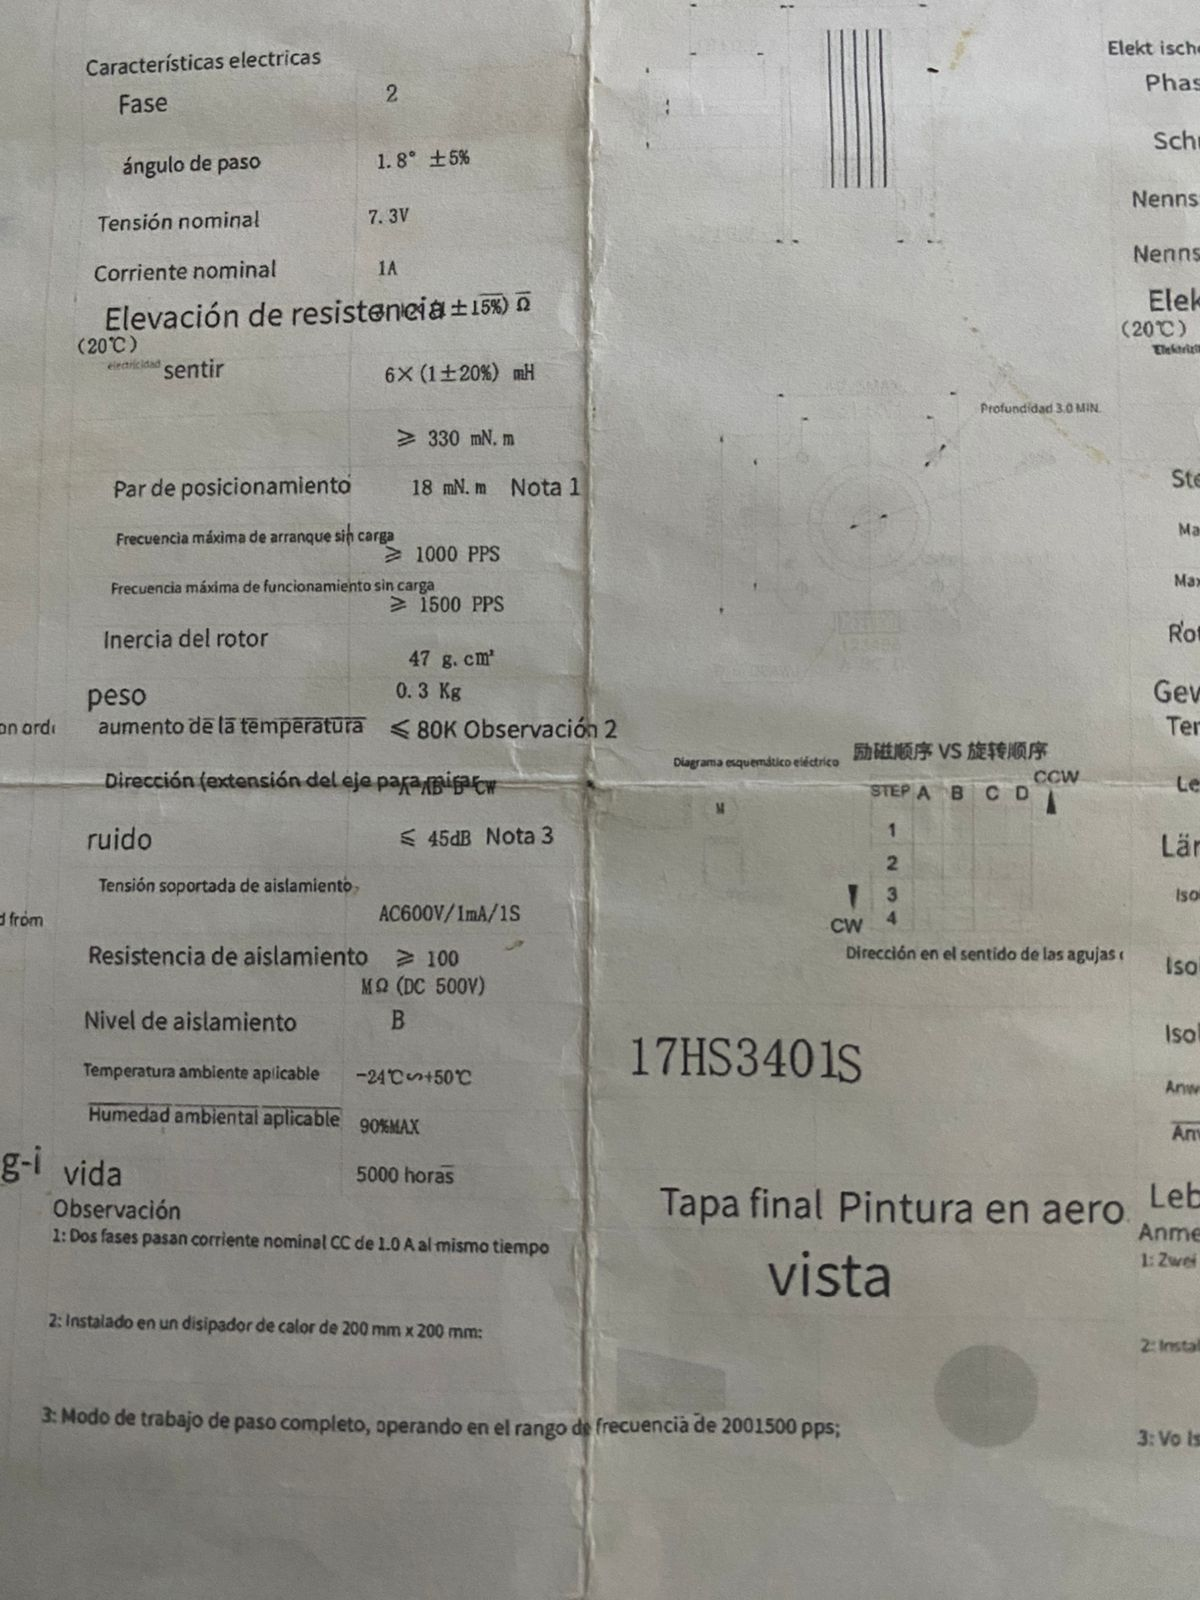
\includegraphics[width=0.8\textwidth]{imagenes/anexos/datasheet_motor.png}
    \caption{Datasheet de un motor stepper bifásico 17HS3401S.} 
    \label{fig:datasheet_motor} % Esta es la "llave" para referenciarlo
\end{figure}

\chapter{Mediciones de inductancia}

\begin{figure}[htbp]
    \centering
    \includegraphics[width=0.8\textwidth]{imagenes/anexos/medicion_inductancia.png}
    \caption{Mediciones de inductancia del motor stepper bifásico 17HS3401S.} 
    \label{fig:medicion_inductancia} % Esta es la "llave" para referenciarlo
\end{figure}
% 4. Bibliografía
\newpage
\addcontentsline{toc}{chapter}{Bibliografía} % Para que aparezca en el índice
\bibliographystyle{ieeetr}
\bibliography{referencias.bib}

\end{document}